\documentclass{article}
\usepackage[utf8]{inputenc}
\usepackage[spanish]{babel}
\usepackage{listings}
\usepackage{graphicx}
\graphicspath{ {Pictures/} }
\usepackage{cite}

\begin{document}

\begin{titlepage}
    \begin{center}
        \vspace*{1cm}
            
        \Huge
        \textbf{Proyecto investigativo}
        
            
        \vspace{0.5cm}
        \LARGE
        Taller nociones de la memoria del computador
            
        \vspace{1.5cm}
            
        \textbf{Luis Fernando Torres Torres}
        
        \vspace{4cm}
            
        \textbf{PhD. Augusto Salazar Jiménez}
            
        \vfill
            
        \vspace{0.8cm}
            
        \Large
        Despartamento de Ingeniería Electrónica y Telecomunicaciones\\
        Universidad de Antioquia\\
        Medellín\\
        Septiembre de 2020
            
    \end{center}
\end{titlepage}

\tableofcontents%Tabla de contenidos 

\newpage

\section{Introducción}\label{intro}
Uno de los componentes más importantes dentro de la computación es la memoria, la cual esta estrechamente relacionada con el concepto de almacenamiento de información y datos que contienen todos los programas.En este documento se introduce de manera clara y sencilla, ciertos conceptos que son de vital importancia para entender la definición, el funcionamiento y tipos de memoria que usa el computador para realizar cualquier proceso o tarea.

\section{Sección de contenido}
\subsection{Que es la memoria del computador.} \label{contenido}
La memoria del computador sin lugar a duda cumple un papel muy importante dentro de la computacion y su funcionamiento,ya que es aquel componente que se encarga almacenar de manera temporal toda la informacion relevante y necesaria que va a ser procesada o usada en dicho computador \cite{augusto}.\\

La memoria almacena toda la infomracion en grupos de bits que se denominan palabras, es decir conjunto de números 1 y 0 que puede representar un número,un caracter,una cadena de texto o cualquier tipo de  información. La capacidad de las memorias en las computadoras comerciales de hoy en dia,se da a conocer en la cantidad de  bytes que pueden almacenar.\cite{arquitectura}\\

Por otra parte ,el funcionamiento de una memoria tiene unas características importantes que clasifica los
diferentes tipos de memoria tal como lo son la localización, la capacidad de almacenamiento, el método de acceso, la organización de los datos en una memoria, el tiempo de acceso y velocidad,entre otros.\\

Es importante reconocer que tipo de memoria usar para una tarea especifica,por lo que dependiendo de sus caracteristicas,es o no util para cierto tipo de memoria como se vera en la seccion \ref{tipos}.Para mayor entendimiento y esclarecer mejor el concepto de que es una memoria,es importante hablar de las caracteristicas que clasifica una memoria.


\begin{itemize}
    \item \textbf{Localización de la memoria}:Esta caracteristica hace referencia basicamente al lugar donde esta pocisionada la memoria dentro del computador,la cual puede estar dentro del procesador como lo es el caso de los registros y memoria cache,memoria interna como la memoria RAM,y memoria externa como lo es el disco duro o unidades opticas.
    
    \item \textbf{Capacidad de la memoria}:Hace referencia a la capacidad de almacenamiento o a la cantidad de informacion que una memoria puede acumular.La unidad de informacion que se usa para medir esta capacidad es el byte.
    
    \item \textbf {Métodos de acceso}: Hace referencia a el metodo que cada tipo tiene memoria tiene para acceder a las pocisiones,como por ejemplo secuencial,el cual se accede desde la ultima posicion que se ha accedido, y continua la busqueda en orden hasta llegar a la pocision deseada,otro metodo es el directo,donde la memoria se divide en bloques y dentro de cada bloque se realiza un acceso secuencial hasta llegar a la pocision deseada,el metodo aleatorio,en el cual la memoria se organiza como un vector, donde cada elemento tiene una unica direccion y se realiza la bsuqueda de manera aleatoria,y por ultimo el metodo asociativo,donde el accceso se realiza no con la direccion de la memoria si no mas bien con el contenido desado , es decir en este metodo se especifica el valor a buscar y el compara el contenido de cada posicion de la memoria con el contenido deseado. 
    \begin{figure}[h]
    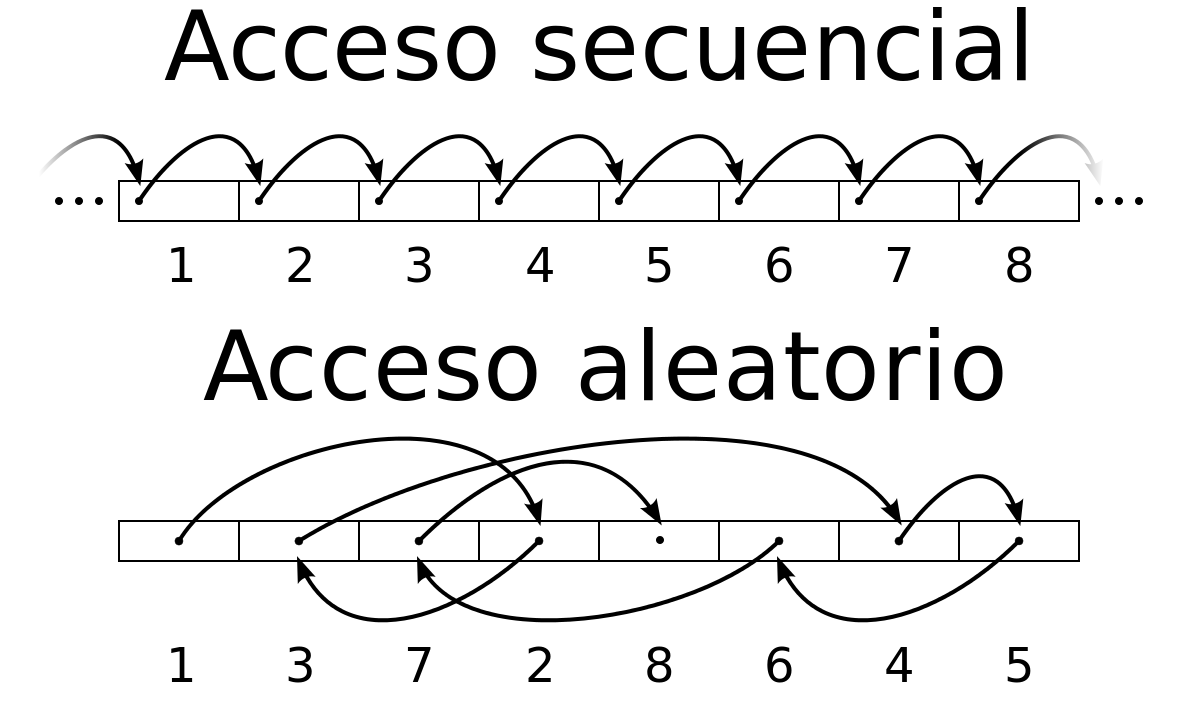
\includegraphics[width=7cm]{accesos.png}
    \centering
    \caption{Acceso secuencial vs aleatorio}
    \label{vs2}
    \end{figure}
    \end{itemize}

\subsection{Tipos de memoria.} \label{tipos}%Explicar usos de cada memoria

En una computadora existen diferentes tipos de memoria cada una con tareas especificas,esto con el fin de realizar de manera mas eficiente y rapida el proceso busqueda y utilizacion de recursos.Dentro de esto se encuentran los siguientes tipos de memoria:

\subsubsection{Memoria ROM}
La memoria ROM (Read Only Memory - Memoria de Sólo Lectura) \cite{augusto}, es conocida como memoria no volátil ya que la información contenida en ella
no es borrable una vez se apague el dispositivo electrónico,en este vital componente se almacenan programas firmware, es decir, programas como el
sistema operativo, intérpretes o compiladores de lenguajes,y otros programas que no necesitan ser modificados actualizados,o alterados constantemente \cite{memorias},ya que como su nombre lo indica,esta unidad  solo posee la operacion de lectura,no tiene posibilidad de escritura.
La memoria ROM se encuentra instalada en la tarjeta madre “motherboard” lugar donde se encuentra la información básica del equipo, llamada “BIOS.”

\subsubsection{Memoria cache}
La memoria chache,es un componente que se caracterisa  principalmente por su alta velocidad de acceso,en orden de jerarquia es la memoria mas rapida, pero a su vez tiene poca capacidad de almacenamiento para datos e información.En esta memoria se almacenan temporalmente los datos que son usados con mayor frecuencia,para asi lograr tener una acceso rapido,casi inmediato\cite{arquitectura}. Dicha memoria caché esta directamente interconectada con el microprocesador y se divide en tres niveles (levels en inglés) L1, L2 y L3. \cite{augusto}, donde a medida que el nivel va aumentando su capacidad de almacenamiento va aumentado tambien y su velocidad de acceso va disminuyendo , es decir la memoria mas veloz pero con menos capacidad es L1, y por el contrario la menos veloz pero con mayor almacenamiento la memoria cache L3.

\subsubsection{Memoria RAM}
La memoria RAM (Random Access Memory -memoria de Acceso Aleatorio),es sin duda la memoria mas conocida e importante del computador,recibe dicho nombre, dado a  que está divida en celdas de memoria, donde se almacenan temporalmente cada uno de los bits o pulsos electricos que contienen toda la informacion con la que trabaja el microprocesador \cite{augusto}.\\

La memoria RAM esta diseñada para optimizar la velocidad de respuesta al momento de utilizar algún
programa en el computador, por lo que  la información que se  necesita para llevar a cavo un proceso  se encuentra almacenada temporalmente en dicha memoria,  en consecuencia, la memoria RAM y el procesador interactúan entre si intercambiando una gran cantidad de datos en poco tiempo.\\

La memoria RAM almacena dicha información y le envía al procesador los datos que necesitan
ser procesados, por lo tanto, mientras la memoria posea mayor velocidad de transmisión y
mayor capacidad de almacenamiento el usuario podrá utilizar más programas a la vez y de
manera más rápida \cite{apuntes}.\\

\noindent
\textbf{DRAM}.\\
Pero llendo mas a fondo, cada una de las celdas de la memoria RAM, a nivel circuital esta constituida por un transistor y un capacitor, que en conjunto realizan un proceso muy importante , el cual consiste basicamente en recargar la memoria constantemente de informacion,por el cual se le denomina DRAM (Dynamic Random Access Memory -Memoria de Acceso Aleatorio Dinámica).Este tipo de memoria dinamica tiene una gran ventaja economica y en capacidad de almacenamiento frente a la memoria chache, pero a su vez,estar refrescando la informacion a cada instante hace que sea un proceso mas  lento \cite{augusto}.\\

\noindent
\textbf{SRAM}.\\
Por otra parte,existe la memoria denomida SRAM (Static Random Access Memory -Memoria de Acceso Aleatorio estatica),que a diferencia de la DRAM es mucho mas veloz y la informacion permanece por un tiempo mas prolongado sin ncesidad de recargarla constantemente,gracias a su cirtcuito interno,que contiene seis transistores y otros componentes,pero como se puede observar, al estar compuesto de mas elementos,ocupa mas espacio en cada celda a comparacion de una DRAM, por lo cual, es economicamente mas costosa, y ademas se obtiene una menor capacidad de almacenamiento.Es por esta razon que la memoria SRAM,es la que se usa en la memoria cache.

\begin{figure}[h]
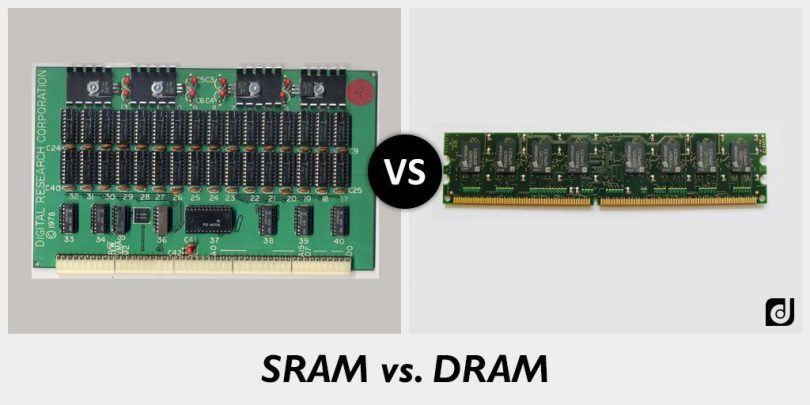
\includegraphics[width=7cm]{vs.jpg}
\centering
\caption{SRAM vs DRAM}
\label{vs}
\end{figure}

\subsubsection{Memoria Virtual}
Después en el nivel de jerarquías la siguiente memoria es la memoria virtual,la cual es una porción del disco duro que se dedica exclusivamente a almacenar temporalmente porciones de los programas y datos que se esten ejecutando,y que ocupan espacio innecesario en algún momento determinado , es decir, que cada vez que haya algún programa ocupando mucho volumen de la memoria RAM , pero que no se está usando,la memoria virtual se encarga de "sostenerlo" hasta próximo aviso con lo cual se aumenta la disponibilidad de almacenamiento en la RAM la cual puede ser utilizada para otros procesos\cite{augusto}.

\subsubsection{Disco Duro}
El disco duro, puede ser considerado como una memoria al igual las nombradas anteriormente,de hecho este es el espacio donde se almacenan permanentemente todos los programas,datos,software e informacion que contiene el computador .A diferencia de las otras memorias,el disco duro tiene la capacidad de conservar toda la informacion almacenada aun despues de apagar el equipo,es decir,es una memoria no volatil.El disco duro al obtener una gran capacidad de almacenamiento en comparacion a las memorias vistas anteriormente, la busqueda dentro de el es muy lenta , lo cual hace que sea ineficiente para ser la memoria principal de un computador \cite{disco}.

\begin{figure}[h]
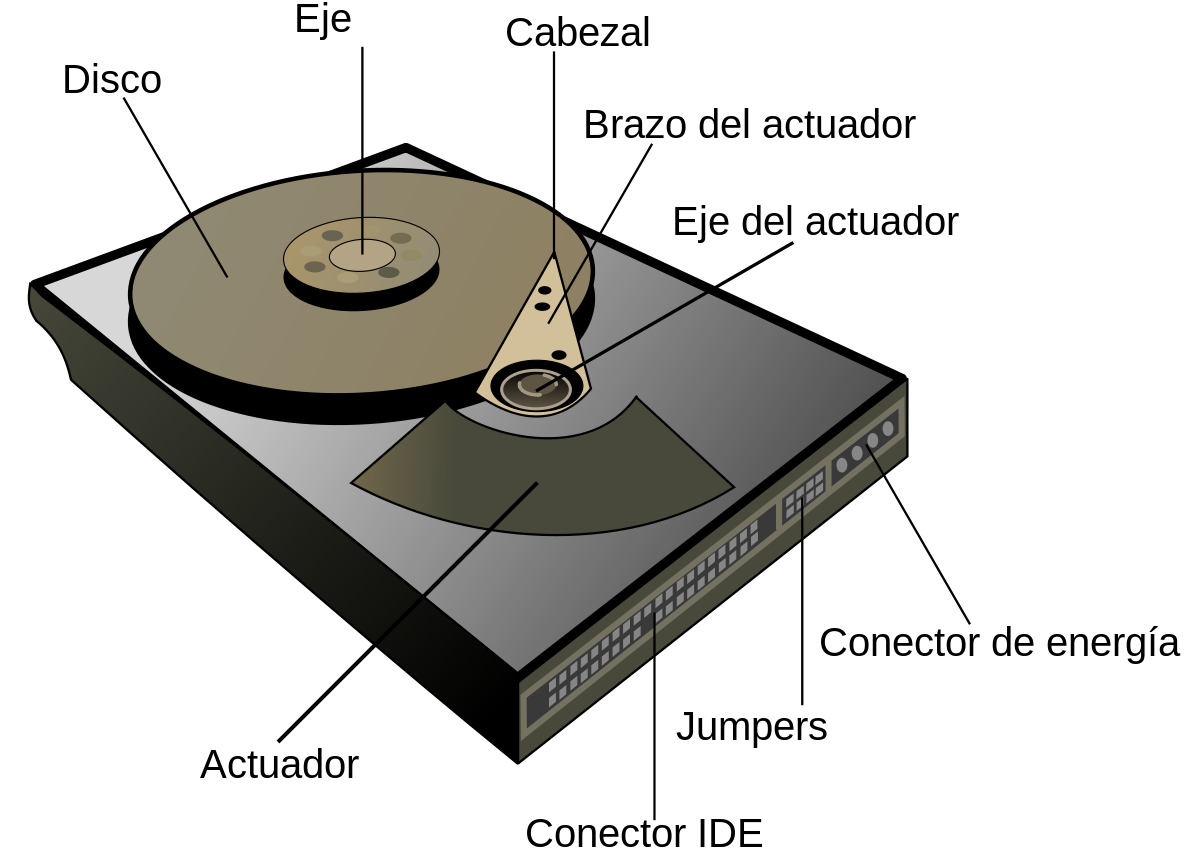
\includegraphics[width=7cm]{HDD.png}
\centering
\caption{Disco Duro}
\label{hdd}
\end{figure}


\subsection{Como se gestiona la memoria en un computador.} \label{contenido}

\subsection{¿Qué hace que una memoria sea más rápida que otra? ¿Por qué esto es importante?}.\label{comparacion}
Como se puedo observar en el literal \ref{tipos}, se hablo de jerarquia de memorias, donde se especifica que unas son mas rapidas que otras,esto se debe a varios factores que tienen que ver  tanto con la parte fisica de los circuitos, la  arquitectura,y la frecuencua con la que funciona cada bus,por ejemplo en el caso del disco duro, al obtener tanta informacion y al tener una arquitectura de disco magnetico,el debe dar toda la vuelta para buscar algo concreto,mientras que en la RAM al estar divida por celdas la informacion se obtiene de manera inmediata,ademas,en el caso de la memoria RAM al tener menos informacion es mas sencillo realizar la busqueda.\\

Por otra parte La memoria SRAM,al funcionar en sincronia con los ciclos de reloj del bus de la motherboard(placa madre),es dependiente de la frecuencia y latencia que se tenga en el sistema.Los cuales estan relacionados con la siguiente exprecion:\\\\

\begin{equation}
\frac{Latencia(CAS)}{Frecuancia(MT/s)}*2*1024 
\label{eq}
\end{equation}
\\\\
Para finalizar,la diferencia de velocidades entre memorias es importante, porque gracias a esto se logra obtener una buena gestion y un buen equilibrio entre velocidad y almacenamiento,ya que el realizar una sola memoria que tenga una velocidad y capacidad muy grande, ademas de ser un proceso bastante costoso,obtendria tamaños no tan portables,es decir se tendria que crear tarjetas madre mucho mas grandes,con circuitos mucho mas capaces que posean gran cantidad de buses,pistas y demas elementos ,lo cual para una empresa no es para nada rentable,al dia de hoy esto se puede notar un poco con el disco de estado solido (SSD-solid state disk), que es mucho mas veloz que un disco duro (HDD-Hard drive disk),pero a su vez tiene un precio mas elevado por la misma cantidad de almacenamiento.Por esta razon es mas viable,crear una gran gama de memorias con tareas y velocidades especificas, para que asi el proceso de fabricacion de un computador se pueda hacer lo mas comercialmente posible.


\section{Conclusiones}.\label{conclusiones}
\begin{itemize}
    \item El proceso para lograr un almacenamiento optimo y eficiente de informacion dentro de un computador, requiere un trabajo arduo,largo y con mucha organizacion;ademas de un estudio colaborativo entre diferentes areas e ingenierias, para lograr una rapidez impresionante y un excelente resutlado.
    \item El conocimineto y saber acerca de como funcionan las memorias en un computador,hace reflioxionar acerca de que tan complejo es el proceso que realizan los dispositivos digitales que usamos a diario tales como smart TV,celulares ,tablets y  computadores.
\end{itemize}

\newpage

\bibliographystyle{IEEEtran}
\noindent
\bibliography{references}

\end{document}